\section{Case study: reference data, conditions and planned analyses}
\label{app:study1}

\subsection{Reference data and its audit}
\label{app:study1-data}
\paragraph{Corpus.}
The corpus holds \NCorpusDocs{} authentic regulatory instruments on rooftop solar from \NCorpusJurisdictions{}
jurisdictions in India: central schemes and the regulations and orders of state commissions and distribution
companies. Superseded instruments stay in the corpus, because their continued availability is the hazard studied.
Every file is hashed and listed with its issuer, dates and source URL.

\paragraph{Amendment registry.}
The reviewer's amendment record is a registry of \NLinksRegistry{} clause-level links, each from an old clause to the
clause that changes it, with a relation (supersedes, partially supersedes, amends), an effective date and a quote from
the amending instrument. It was extracted from the documents by an AI assistant, without access to the gold graph (the
adjudicated replacement links used for scoring). It is the source of the \rung{R3} quotes, the \rung{R4} and \rung{R4n} status lines and the \rung{R5}
lookup. The registry as corrected by adjudication (below) is the one every run uses.

\paragraph{Cases and reference answers.}
A case is a synthetic application: an electricity bill, an installer proposal and a distribution-company portal record,
with a case date and a jurisdiction. Cases were generated backward from rule functions whose parameters are quoted from
the clause text, so no label was typed by hand. Each case records the rule function that labelled it; most cases list a
single applicable rule. The applications contain no personal data. The candidate test set had \NCandidateCases{} cases
on the replaced clauses with enough fixed answers per condition; the dev split shares no replaced clause with it and was
used only for engineering and the pilot.

\subsubsection{Human audit of the reference data}
\label{sec:annotation}
The registry, the answer key and the case labels were produced with AI help, so two authors checked them blind before
the test set was sealed, splitting the work and labelling a seeded shared subset (\NSharedCases{} cases, \NSharedLinks{}
links) in common. They labelled each case's decision, blocking stage and deciding clauses from the case file and the
source documents; each checked link's relation, effective date and wording; and a sample of \NControlsAnnotated{} matched
correct answers. A third author, who led the pipeline that produced the first-pass labels, adjudicated every
disagreement from the annotators' sheets and the source documents, without the answer keys. The planned procedure
had the annotators meet first; to save time the meeting was dropped and all disagreements went to the adjudicator
(Appendix~\ref{app:deviations}). The annotators are not legal professionals.

On the shared cases the annotators agreed on the decision in \AgreeCasesDecision{} of cases (kappa
\KappaCasesDecision{}) and on the blocking stage in \AgreeCasesBlockingStage{} (kappa \KappaCasesBlockingStage{}), but on
the exact set of deciding clauses in only \AgreeCasesDecidingClauses{} (kappa \KappaCasesDecidingClauses{}). On shared
links they agreed on the relation in \AgreeLinksRelation{} (kappa \KappaLinksRelation{}). Part of the clause-level
disagreement is notation (\cfg{cl-4.2} against \cfg{cl-4(2)}); part is that several clause sets support the same outcome.

\paragraph{The answer key.}
Against the adjudicated labels, the AI-built key reached a different outcome on \NDroppedDecision{} of the
\NCandidateCases{} cases: \NDroppedDecisionOnly{} on the decision and \NDroppedBlockingStage{} on the blocking stage of a
rejection. In the disagreements we inspected, the readers based their decision on a second clause that the case's rule
function does not evaluate, often in a newer instrument. In one such case, the key approves an application because it passes the
transformer-capacity rule its rule function checks; the readers reject it under an eligibility clause of a later
regulation. These cases are wrong at the base, and they are dropped; a case is never relabelled, because its faults
were planted on the key's answer. On \NClauseDisputed{} of the remaining cases, the outcome agrees and only the deciding
clauses differ. Those cases are kept and listed, because a planted fault and its catch are defined on the replaced
clause alone. Applied as originally planned, which dropped clause-only disputes too, the rules would have kept
\NStrictKept{} cases.

\paragraph{The correct answers.}
Of the \NControlsChecked{} matched correct answers checked, \NControlsCorrect{} (\PctControlsCorrect) were judged correct.
Most of the rest were judged incomplete or citing a wrong clause, the same single-rule cause: they cite the clause the
rule function evaluated and omit another that also decides the case. A reviewer that flags such an answer may be right,
so these items bias false alarms upwards. The planned gate (\ControlsGatePct\% correct) would have stopped the seal; it
was replaced by reporting, and by sensitivity set S1, which removes every case whose checked correct answer was judged
anything but correct (\S\ref{sec:setup}).

\paragraph{The registry.}
The \NLinksAnnotated{} checked links are the \NLinksUsed{} that test items rely on and a seeded \LinkSamplePct\% random
sample of \NLinksSample{} of the other links. In the random sample, \NLinksSampleConfirmed{} were confirmed,
\NLinksSampleRelChanged{} had a different relation, and \NLinksSampleNotALink{} were judged to be no change at all
(\CINotALinkSample{}, Wilson 95\% interval). Among the test-item links, \NLinksTestPairNotALink{} was no change and
\NLinksTestPairRelChanged{} had a different relation. Rejected links were removed and corrected dates applied before
the run. These figures describe links the registry asserts. Nothing in the audit looked for links the registry misses,
so we do not estimate that rate. The full table, with both annotators' raw answers beside the adjudicated one, is
released (\cfg{40\_data/link\_audit\_v1}); links outside the check keep the extractor's provisional relation and are not
used as gold.

\paragraph{The scorer.}
One annotator labelled \ScorerCheckN{} dev replies by hand under the written scoring rule. The automatic scorer agreed on
\ScorerCheckAgreeN{} (\ScorerCheckPctObserved), below the planned \ScorerCheckPct\% gate. In each of the
\NScorerDisagree{} disagreements, the reply's own clause ids and reason codes give the scorer's label under the written
rule, so the scorer was not changed. Most disagreements lie on the boundary between a wrong clause and a wrong reason
(\NScorerClauseReason{}), or between a right catch and a wrong reason (\NScorerCatchReason{}). We read this as evidence
that the right-reason rule is hard to apply by hand, not as a defect of the scorer, and report every result under the
two looser rules as well (E5).

\paragraph{The sealed test set.}
The sealed set has \NTestCases{} cases on \NClauses{} distinct replaced clauses from \NStates{} jurisdictions
(Table~\ref{tab:items}). They come from \InstrNIntactGemma{} amending instruments (\NSharedInstrument{} clauses in one
state from a single one), so clauses are not independent. The registry links \NRegistryFlagged{} of the \NClauses{} replaced clauses; on the others the intact
registry itself reads \cfg{in\_force}, so they are naturally missing links.

\begin{table}[t]
\centering
\small
\begin{tabular}{lrrr}
\toprule
Condition & Faults & Matched correct answers & Clauses \\
\midrule
S-both (old and current clause shown) & \NFaultsSBoth & \NControlsSBoth & \NClausesSBoth \\
S-swap (old clause in place of current) & \NFaultsSSwap & \NControlsSSwap & \NClausesSSwap \\
C (clean correct answers) & -- & \NCleanC & -- \\
\bottomrule
\end{tabular}
\caption{Fixed answers per condition in the sealed test set. Clauses: distinct replaced clauses. Jurisdictions of the
replaced clauses: DL \NClausesStateDL, GJ \NClausesStateGJ, central \NClausesStateIN, KA \NClausesStateKA,
TN \NClausesStateTN, UP \NClausesStateUP.}
\label{tab:items}
\end{table}

\subsection{Conditions, damage and scoring}
\label{app:study1-conditions}
\label{sec:method}

\subsubsection{Fixed answers}
\label{sec:probe}
We measure review on fixed answers, so the result does not depend on what a generator happens to write. For each case
and condition we build a matched pair. The \emph{fault} cites the replaced clause in place of its successor. When the old
clause changes the approve-or-reject outcome, the fault also carries the decision that clause implies; otherwise it has
the right decision on an invalid basis. The \emph{matched correct answer} (control) has the key's decision and cites only
clauses its own evidence shows. Both come from one neutral template: the decision, the cited clause identifiers, one
sentence that quotes the basis clause, and the blocking stage if any. A pair therefore differs only in its basis and,
where the outcome changes, in the decision. Condition C adds one clean correct answer per case. The reviewer sees the
case, the evidence and one answer, and is never told which answers are faults.

The evidence differs by condition. In \emph{S-both} the old clause and its successor are both shown; in \emph{S-swap}
the old clause replaces the current one, so the reviewer sees only outdated text.

\subsubsection{Conditions}
\label{sec:conditions}
Every language-model condition uses the same validity prompt, which asks whether each cited clause is in force on the
application date, issued for the case's jurisdiction and applicable to its facts. Conditions differ only in what the
prompt contains (Table~\ref{tab:conditions}; prompts in Appendix~\ref{app:prompts}). \rung{R3}, \rung{R4} and \rung{R4n}
are built on \rung{R2}: the \rung{R3} block holds the amending instrument's verbatim substitution text for each cited
clause the registry links, with no status, date or target; the \rung{R4} block holds one line per cited clause giving
the registry's entries, jurisdiction and status at the case date. \Rfourp{} gives the same line at \rung{R1}, without
the current clause; it shows what the status line does when the text cannot confirm it. \rung{R5} uses no language
model: it raises a ``not in force'' finding on a cited clause exactly when the registry marks that clause superseded or
partially superseded at the case date (an ``amends'' link alone does not), and it raises no other kind of finding. Its
catches are therefore the registry's own links, and its false alarms are the registry's own wrong links.

\paragraph{The no-record arm.}
In the registry, a clause with no outgoing link has status \cfg{in\_force}. The registry cannot distinguish a clause
that was never amended from one whose amendment it failed to record, so this value states more than the record holds.
\rung{R4n} replaces the status value \cfg{in\_force} by \cfg{no\_\allowbreak amendment\_\allowbreak recorded} and changes nothing else: the
prompt sent at \rung{R4n} equals the \rung{R4} prompt with that one substitution, which a unit test checks on an
intact and a damaged registry. Superseded, partially superseded and not-yet-in-force values are unchanged. The substitution applies to every clause
the registry does not link, including current clauses on correct answers, so \rung{R4n} can change false alarms as well as
catches.

\begin{table}[t]
\centering
\scriptsize
\setlength{\tabcolsep}{3pt}
\begin{tabular}{p{1.45cm}p{2.85cm}p{2.2cm}p{2.95cm}p{1.5cm}}
\toprule
Condition & Reviewer sees & Reviewer does not see & Compared with; confound & Role \\
\midrule
\rung{R0} & old clause (S-swap), source metadata removed & current clause, dates, issuer & -- & ladder \\
\rung{R1} & old clause with issuer, dates, title & current clause & \rung{R0}: metadata only & ladder \\
\rung{R2} & old and current clause (S-both) & any amendment record & \rung{R1}: adds the current clause & ladder; Q2 baseline \\
\rung{R3} & \rung{R2} + amending instrument's words & status, dates, target & \rung{R2} & ladder \\
\rung{R4} & \rung{R2} + registry status line & -- & intact: told the answer for linked clauses & reference \\
\Rfourp{} & \rung{R1} + registry status line & current clause & \rung{R1}: status line without the text & ladder \\
\rung{R4}-damage & \rung{R2} + status line of a damaged registry & which links are wrong & \rung{R5}-damage (Q1); \rung{R2} (Q2) & primary \\
\rung{R4n}, \rung{R4n}-damage & as \rung{R4}, ``no amendment recorded'' for unlinked clauses & -- & \rung{R4} on the same items and seeds & primary \\
\rung{R5}, \rung{R5}-damage & no LLM: ``not in force'' on every cited clause the registry marks superseded & -- & catches exactly the linked clauses, by construction & reference \\
\bottomrule
\end{tabular}
\caption{Conditions. ``Reference'' rows are not findings: \rung{R5} recovers the registry's own links, and \rung{R4} at the
intact registry is told, for every linked clause, that it is not in force. Faults were planted on replaced clauses of the
gold graph; the registry links most but not all of them (\S\ref{app:study1-data}). The E2 variants of \rung{R0} to
\rung{R2} add a ``can't confirm'' reason.}
\label{tab:conditions}
\end{table}

\paragraph{Can't confirm.}
For E2, variants of \rung{R0}, \rung{R1} and \rung{R2} add the reason \cfg{currency\_unconfirmed}: the evidence shown does
not establish whether the clause is in force at the case date. Such a finding is neither a catch nor a false alarm.

\subsubsection{Damaged registries}
\label{sec:damage}
To vary the record's reliability in a controlled way we damage the registry in three ways: \DamageDropTwentyFive\% or
\DamageDropFifty\% of its links dropped, or \DamageSpuriousTen\% spurious links added. Each damage has \NDamageSeeds{}
seeds. A drop permutes all of the registry's links with the seed and removes the first quarter or half, so at one seed
the 50\% set contains the 25\% set. A spurious link is added from a seeded choice of dated clauses that have no
outgoing link, to another clause of the same jurisdiction, as a ``superseded by'' link effective from the clause's own
date; the number added is 10\% of the registry's links. A damaged registry is used in each way the intact one is: as the lookup
(\rung{R5}-damage) and as the status line (\rung{R4}-damage, \rung{R4n}-damage). A dropped link makes the status line
report a replaced clause as \cfg{in\_force} (\rung{R4}) or as having no recorded amendment (\rung{R4n}), while the evidence
still shows both versions; a spurious link makes it report a current clause as replaced. In both cases the text in view
contradicts the line. The damage is random and synthetic; it is not an estimate of how real registries fail.

\subsubsection{Scoring}
\label{sec:scoring}
The reviewer returns a verdict and findings; each finding names a clause and gives one reason from a closed list (not in
force, wrong jurisdiction, not applicable, missing rule, content or arithmetic, other). The list is the same in every
prompt and names no clause.

\paragraph{Catch, false alarm, confusion counts.}
A fault is caught when a finding names the replaced clause with the reason ``not in force''; an identifier of a
retrieval chunk counts as the clauses it contains. On a correct answer, any finding is a false alarm. Each condition
therefore yields four counts: caught and missed faults, flagged and passed correct answers. A finding on the right clause
for another reason is not a catch; we count it as a \emph{misnamed} alarm (E4).

\paragraph{Discrimination.}
For one replaced clause, discrimination is its catch rate on faults minus the false-alarm rate on their matched correct
answers; it is averaged over clauses, and for a damaged registry first over seeds within a clause. It is the headline
measure, because a reviewer that flags every answer catches every fault and is of no use.

\paragraph{Deference and NoRec.}
Both use the same items: every (S-both fault, drop rate, seed) where the intact registry catches the fault and that
damaged registry does not. Deference is, item by item, the reviewer's catch with no registry (\rung{R2})
minus its catch with the damaged status line (\rung{R4}-damage). NoRec is the item's catch at \rung{R4n}-damage minus its
catch at \rung{R4}-damage on the same seed. Both are averaged within clause, then over clauses.

\paragraph{Three scoring rules (E5).}
Under \emph{any finding}, a fault is caught if the reply has any finding; under \emph{clause named}, if a finding names
the replaced clause for any reason; the right-reason rule above is the strictest. On correct answers we report any finding
(our false-alarm rule) and a finding with a validity reason only.

\paragraph{Post hoc measures.} These were added after the results were seen and were not pre-specified.
Because the lookup can only raise ``not in force'' while the reviewer can raise any reason, we also report Q1 with false
alarms counted only when the finding gives a validity reason (not in force, wrong jurisdiction, not applicable), the
reason codes behind the false alarms, the catches the reviewer gains and loses against the lookup on the same item and
seed, and Q1 with the amending instrument rather than the clause as the unit (the \NClauses{} clauses come from fewer
amending instruments). These are descriptive and outside the family.

\paragraph{Invalid replies.}
A reply that is not valid JSON, is cut off at the output cap after one retry, or has no verdict is invalid. It counts as a
miss on a fault and as a false alarm on a correct answer, so an invalid reply never improves a condition.

\subsection{Setup and planned analyses}
\label{app:study1-planned}
\label{sec:setup}

\paragraph{Models.}
The panel has \NPanelModels{} open models: \texttt{llama3.1:8b} (weak), \texttt{qwen2.5:7b}, and the \NCapable{} capable
models \texttt{qwen2.5:14b} and \texttt{gemma-4-26b-a4b-it}. The first three run through Ollama with 4-bit quantised
weights fixed in advance by digest (\texttt{46e0c10c039e}, \texttt{845dbda0ea48} and \texttt{7cdf5a0187d5}; full digests
in the analysis plan), checked on every machine: \texttt{qwen2.5:14b} on a cloud notebook with two NVIDIA T4 GPUs, the
other two on an Apple-silicon laptop. Gemma, open-weight, runs through a hosted API, with the version recorded per call.
A closed hosted model, \texttt{gemini-3.5-flash-lite}, is a secondary model on \rung{R0}, \rung{R2} and \rung{R4} only.
Each model ran on one machine. Models added after the plan was fixed are exploratory and reported separately
(\S\ref{sec:res-explore}).

\paragraph{Settings.}
Decoding is greedy (temperature \Temperature), with run seed \RunSeed{} and an output cap of \OutputCap{} tokens. Every
reply is cached, and every block records the model digest, the prompt hash per item, the code hash and the hash of the
sealed test file. Every model sees the same items.

\paragraph{Run order and cutoff.}
Blocks run in a fixed priority order: for the capable models \rung{R2}, \rung{R4}, \rung{R4n}, \rung{R5} and
\rung{R5}-damage, then \rung{R4}-damage and \rung{R4n}-damage seed by seed, so that a cut run still leaves the two arms
paired on the same seeds; then the secondary conditions; then the other models. The analysis cutoff was fixed as a
wall-clock time before any test result was read. A block not finished by then is reported as not run, and a contrast whose blocks are
incomplete is reported as not run rather than estimated from part of a block; every planned block finished
(Appendix~\ref{app:deviations}).

\paragraph{Unit of inference and tests.}
The unit of inference is the distinct replaced clause. Rates are averaged within each clause and then over clauses, with
pooled counts beside each rate; false alarms on condition C are averaged by rule group, because C plants nothing. A
contrast is the mean per-clause difference, paired by clause within one model, tested with a two-sided sign-flip test over
clauses (exact for few clauses, otherwise \NPermutations{} random sign vectors with a fixed seed). Intervals are
\CILevel\% bootstrap intervals over clauses, printed only with at least \MinClauses{} clauses. A cell with fewer than
\SparseItems{} items or \SparseClauses{} clauses is printed as counts.

\paragraph{Primary family.}
\NPrimaryTestsVFive{} tests, Holm-corrected at $\alpha=\Alpha$: for each capable model, \rung{R4} minus \rung{R5}
discrimination at the intact, \DamageDropFifty\%-drop and \DamageSpuriousTen\%-spurious registries (Q1), deference (Q2) and
NoRec. A contrast on fewer than \MinClauses{} clauses enters the family with $p=1$. The \DamageDropTwentyFive\% drop is
reported beside Q1, uncorrected. Everything else is secondary and uncorrected or descriptive: the ladder contrasts (E1),
can't confirm (E2), spurious-link false alarms (E3$'$), misnamed alarms (E4), the scoring rules (E5), the false-alarm cost
of \rung{R4n}, and descriptive splits by amendment wording (explicit or implicit), by whether the fault changes the
outcome, and by cost per call (tokens and seconds).

\paragraph{Sensitivity sets.}
Every primary result is also computed on two subsets, with the same tests and outside the family. S1 removes
every case whose checked correct answer was judged anything but correct. S2 removes every case the originally
planned rule would have dropped, that is, every case whose deciding clauses differ from the key; it has fewer than
\MinClauses{} clauses and is descriptive. Only a sample of correct answers was checked, so S1 removes the correct
answers known to be flawed, not every flawed one; a result that keeps its sign under S1 does not depend on those.

\paragraph{Damage seeds.}
The capable models run \rung{R4}-damage and \rung{R4n}-damage on all \NDamageSeedsCapable{} seeds; the other models run
seed 0. \rung{R5}-damage is deterministic and runs every seed.

\paragraph{Analysis plan.}
The design, outcomes, analysis and the sentence reporting each outcome were written into a dated, version-controlled
analysis plan before any model saw a test item, and the test set was sealed with a fingerprint recorded in the
repository. The plan was not filed with a public registry; the commit times of the plan and its amendments are listed in the release's provenance file. Two dated
amendments were made before the seal. The first, written after the dev pilot, made the
damaged-registry comparisons primary. The second, written after the human audit and before any model saw a test item,
changed which cases annotation keeps, replaced the correct-answer and scorer gates by reporting, and added \rung{R4n},
NoRec, S1 and S2 (Appendix~\ref{app:deviations}).

\subsection{Planned results}
\label{app:study1-results}

Seven reviewers ran on the same items: the five planned models, and two added after the analysis plan was fixed,
\texttt{qwen2.5:32b} (damage seeds 0--2) and Claude Opus~4.5 through a hosted proxy (damage seed 0; temperature and
seed set by the proxy). Every planned block finished for the planned models.
Table~\ref{tab:main} gives the confusion counts of every main arm on the same \NFaultsSBoth{} S-both faults and
\NControlsSBoth{} matched correct answers. A repeat of \texttt{qwen2.5:14b}'s \rung{R2}, \rung{R4} and \rung{R4n}
blocks on the same machine with an empty cache returned identical findings on \NRepeatSameFindings{} of
\NRepeatItems{} items; we did not test whether replies are identical across machines or for the hosted models. Invalid replies were rare (Gemma: \InvalidKNGemmaRFourDropFifty{} at
\rung{R4} with \DamageDropFifty\% of links dropped; \texttt{qwen2.5:14b}: none).

\IfFileExists{generated/tab_main.tex}{\begin{table*}[t]\centering\scriptsize
\caption{Main results on S-both faults and their matched correct answers. TP: right-reason catches of the planted superseded clause; FN: faults not caught; FP: matched correct answers with any finding; TN: matched correct answers passed. Recall, specificity, precision and balanced accuracy (\%) pool items, which share clauses, so they are descriptive. FA$_C$: clean correct answers flagged. Disc.: discrimination (catch minus matched false alarm), clause-averaged, with a 95\% bootstrap interval over clauses (points). R5 recovers the registry's own links by construction and R4 (intact) is given the answer: reference rows.}
\label{tab:main}
\resizebox{\textwidth}{!}{%
\begin{tabular}{lllrrrrrrrrrll}
\toprule
Model & Arm & Reviewer sees & TP & FN & FP & TN & Rec. & Spec. & Prec. & Bal. & FA$_C$ & Disc. [95\% CI] & Cl. \\
\midrule
Qwen 14B & R2 & both versions & 13 & 29 & 18 & 24 & 31 & 57 & 42 & 44 & 12/42 & $-$7 [$-$38, +20] & 14 \\
Qwen 14B & R4 & status line & 32 & 10 & 10 & 32 & 76 & 76 & 76 & 76 & 11/42 & +55 [+26, +79] & 14 \\
Qwen 14B & R4n & no-record wording & 31 & 11 & 13 & 29 & 74 & 69 & 70 & 71 & 12/42 & +47 [+17, +73] & 14 \\
Lookup & R5 & lookup (ref.) & 31 & 11 & 5 & 37 & 74 & 88 & 86 & 81 & 5/42 & +67 [+43, +88] & 14 \\
Qwen 14B & R4-drop50 & status, drop 50\% & 88 & 122 & 54 & 156 & 42 & 74 & 62 & 58 & 55/210 & +21 [$-$6, +48] & 14 \\
Qwen 14B & R4n-drop50 & no-record, drop 50\% & 95 & 115 & 58 & 152 & 45 & 72 & 62 & 59 & 60/210 & +23 [$-$6, +54] & 14 \\
Lookup & R5-drop50 & lookup, drop 50\% & 88 & 122 & 8 & 202 & 42 & 96 & 92 & 69 & 8/210 & +42 [+24, +60] & 14 \\
Qwen 14B & R4-spurious10 & status, spur. 10\% & 160 & 50 & 55 & 155 & 76 & 74 & 74 & 75 & 61/210 & +53 [+25, +76] & 14 \\
Lookup & R5-spurious10 & lookup, spur. 10\% & 155 & 55 & 34 & 176 & 74 & 84 & 82 & 79 & 34/210 & +62 [+37, +84] & 14 \\
Gemma 4 26B & R2 & both versions & 9 & 33 & 20 & 22 & 21 & 52 & 31 & 37 & 17/42 & $-$20 [$-$46, +4] & 14 \\
Gemma 4 26B & R4 & status line & 25 & 17 & 20 & 22 & 60 & 52 & 56 & 56 & 18/42 & +21 [$-$18, +57] & 14 \\
Gemma 4 26B & R4n & no-record wording & 26 & 16 & 21 & 21 & 62 & 50 & 55 & 56 & 15/42 & +18 [$-$20, +54] & 14 \\
Gemma 4 26B & R4-drop50 & status, drop 50\% & 89 & 121 & 100 & 110 & 42 & 52 & 47 & 47 & 90/210 & +4 [$-$30, +35] & 14 \\
Gemma 4 26B & R4n-drop50 & no-record, drop 50\% & 96 & 114 & 105 & 105 & 46 & 50 & 48 & 48 & 72/210 & +2 [$-$31, +31] & 14 \\
Gemma 4 26B & R4-spurious10 & status, spur. 10\% & 125 & 85 & 103 & 107 & 60 & 51 & 55 & 55 & 94/210 & +20 [$-$20, +56] & 14 \\
\bottomrule
\end{tabular}}
\end{table*}
}{}

\subsubsection{Q1: does the reviewer add anything over the record?}
\label{sec:res-q1}

\begin{table*}[t]
\centering
\footnotesize
\setlength{\tabcolsep}{3pt}
\begin{tabular}{l ccc ccc}
\toprule
& \multicolumn{3}{c}{\texttt{qwen2.5:14b}} & \multicolumn{3}{c}{\texttt{gemma-4-26b}} \\
\cmidrule(lr){2-4}\cmidrule(lr){5-7}
Registry & \rung{R4} & \rung{R5} & \rung{R4}$-$\rung{R5} & \rung{R4} & \rung{R5} & \rung{R4}$-$\rung{R5} \\
\midrule
Intact & \DiscRFourIntactQwenFourteen & \DiscRFiveIntactQwenFourteen & \DiffNetIntactQwenFourteen & \DiscRFourIntactGemma & \DiscRFiveIntactGemma & \DiffNetIntactGemma \\
Drop \DamageDropTwentyFive\% & \DiscRFourDropTwentyFiveQwenFourteen & \DiscRFiveDropTwentyFiveQwenFourteen & \DiffNetDropTwentyFiveQwenFourteen & \DiscRFourDropTwentyFiveGemma & \DiscRFiveDropTwentyFiveGemma & \DiffNetDropTwentyFiveGemma \\
Drop \DamageDropFifty\% & \DiscRFourDropFiftyQwenFourteen & \DiscRFiveDropFiftyQwenFourteen & \DiffNetDropFiftyQwenFourteen & \DiscRFourDropFiftyGemma & \DiscRFiveDropFiftyGemma & \DiffNetDropFiftyGemma \\
Spurious \DamageSpuriousTen\% & \DiscRFourSpuriousTenQwenFourteen & \DiscRFiveSpuriousTenQwenFourteen & \DiffNetSpuriousTenQwenFourteen & \DiscRFourSpuriousTenGemma & \DiscRFiveSpuriousTenGemma & \DiffNetSpuriousTenGemma \\
\bottomrule
\end{tabular}
\caption{Discrimination in points of the LLM reviewer with the status line (\rung{R4}) and of the registry lookup
alone (\rung{R5}), by registry state, over \NClauses{} clauses. The difference is the Q1 contrast; intervals and
Holm $p$ are in Table~\ref{tab:provenance}. The \DamageDropTwentyFive\% row is outside the primary family.}
\label{tab:q1}
\end{table*}

\IfFileExists{generated/tab_provenance.tex}{\begin{table*}[t]\centering\small
\caption{Primary contrasts (capable models; Holm over the family of ten). Per-clause differences in points, mean over clauses, 95\% bootstrap interval over clauses, two-sided sign-flip test. S1: without the cases whose checked correct answer was judged flawed; S2: under the original strict annotation rule (descriptive when it leaves fewer than ten clauses).}
\label{tab:provenance}
\resizebox{\textwidth}{!}{%
\begin{tabular}{llrrlrrr}
\toprule
Model & Contrast & Clauses & Diff. & 95\% CI & $p$ (Holm) & S1 & S2 \\
\midrule
Gemma 4 26B & Q1, intact: R4 $-$ R5 discrimination & 14 & $-$45 & [$-$69, $-$24] & 0.043 & $-$47 & $-$50 \\
Gemma 4 26B & Q1, 50\% dropped & 14 & $-$38 & [$-$65, $-$11] & 0.178 & $-$38 & $-$50 \\
Gemma 4 26B & Q1, 10\% spurious & 14 & $-$42 & [$-$66, $-$22] & 0.043 & $-$45 & $-$45 \\
Gemma 4 26B & Q2: R2 $-$ R4-damage catch, dropped links & 9 & +1 & -- & 1.000 & +4 & -- \\
Gemma 4 26B & R4n $-$ R4 catch, dropped links & 9 & +9 & -- & 1.000 & +20 & -- \\
Qwen 14B & Q1, intact: R4 $-$ R5 discrimination & 14 & $-$11 & [$-$33, +9] & 1.000 & $-$12 & +17 \\
Qwen 14B & Q1, 50\% dropped & 14 & $-$21 & [$-$38, $-$6] & 0.206 & $-$17 & +2 \\
Qwen 14B & Q1, 10\% spurious & 14 & $-$10 & [$-$30, +10] & 1.000 & $-$11 & +17 \\
Qwen 14B & Q2: R2 $-$ R4-damage catch, dropped links & 9 & +34 & -- & 1.000 & +33 & -- \\
Qwen 14B & R4n $-$ R4 catch, dropped links & 9 & +9 & -- & 1.000 & +9 & -- \\
\bottomrule
\end{tabular}}
\end{table*}
}{}

Under the planned rule, the reviewer given the record had a lower point estimate of discrimination than a lookup
in the same record at every registry state, for both capable models (Table~\ref{tab:q1}). For Gemma the difference
was \DiffNetIntactGemma{} points with the registry intact (CI \CINetIntactGemma, Holm $p=$ \PHolmNetIntactGemma) and
\DiffNetSpuriousTenGemma{} with spurious links (CI \CINetSpuriousTenGemma, Holm $p=$ \PHolmNetSpuriousTenGemma),
both significant after Holm, and \DiffNetDropFiftyGemma{} with half the links dropped (Holm $p=$
\PHolmNetDropFiftyGemma). For \texttt{qwen2.5:14b} it was \DiffNetIntactQwenFourteen{} (Holm $p=$
\PHolmNetIntactQwenFourteen), \DiffNetDropFiftyQwenFourteen{} (CI \CINetDropFiftyQwenFourteen, Holm $p=$
\PHolmNetDropFiftyQwenFourteen) and \DiffNetSpuriousTenQwenFourteen{} (Holm $p=$ \PHolmNetSpuriousTenQwenFourteen),
none significant. The reading fixed in advance for both models is that the reviewer did not discriminate better than a
lookup in the registry it was given, even when the registry was damaged; the reading fixed in advance for Gemma's intact
result is that adding the reviewer to a correct registry made review worse than the registry alone.

That last reading should be taken narrowly, for three reasons we found after the run (post hoc, \S\ref{sec:scoring}).
First, the gap is made of findings the lookup cannot raise. The planned false-alarm rule counts any finding on a
correct answer, but the lookup only ever says ``not in force''. Most of Gemma's findings on matched correct answers gave
``content or arithmetic'' or ``missing rule'' as the reason, not a validity reason. Counting only validity-reason
findings as false alarms, the difference is \DiffNetVIntactGemma{} points for Gemma with the registry intact (CI
\CINetVIntactGemma) and \DiffNetVDropFiftyGemma{} with half the links dropped; for \texttt{qwen2.5:14b} it is
\DiffNetVIntactQwenFourteen{} and \DiffNetVDropFiftyQwenFourteen{} (CI \CINetVDropFiftyQwenFourteen). On the
question the lookup answers, whether a cited clause is in force, the reviewer did about as well as the lookup, except perhaps \texttt{qwen2.5:14b} with half the links dropped, whose
bootstrap interval ends just below zero (the printed 0 is rounded) although its sign-flip test does not reject. The
reviewers' other findings may be right: the audit found that many correct answers omit a clause that also decides the case
(\S\ref{sec:annotation}), which this design cannot score. Second, the \NClauses{} clauses come from
\InstrNIntactGemma{} amending instruments; with the instrument as the unit, Gemma's intact and spurious differences
have uncorrected sign-flip $p=$ \InstrPIntactGemma{} and \InstrPSpuriousTenGemma, on fewer units than the planned
minimum of \MinClauses. Third, both lose significance under S1 (\S\ref{sec:res-sens}). We therefore report Gemma's
Q1 result as planned, but do not read it as evidence that a reviewer degrades a correct record.

The expectation fixed in advance for Q1, that the gap would narrow or reverse as links were dropped because the reviewer
can still read both versions, was not met. Table~\ref{tab:main} shows why. With \DamageDropFifty\% of links
dropped, the reviewer's right-reason catches on S-both faults nearly equal the lookup's for both models. Item by item
and seed by seed, Gemma caught \RecGainedDropFiftyGemma{} faults the damaged lookup missed and missed
\RecLostDropFiftyGemma{} it caught; \texttt{qwen2.5:14b} gained \RecGainedDropFiftyQwenFourteen{} and lost
\RecLostDropFiftyQwenFourteen. The reviewer recovered some dropped links from the text, and lost about as many
catches elsewhere, so on net it did not repair the record. Its false alarms on matched correct answers stayed well
above the lookup's.

Two properties of the design limit this result. The lookup's catches are the registry's own links: it misses
the faults on clauses the registry does not link and flags whatever a wrong link marks, so its discrimination is a
property of the record, not a benchmark of reasoning (\S\ref{sec:method}). And the result holds for these models,
these \NClauses{} clauses and fixed answers with a single planted fault.

\subsubsection{Q2: does the reviewer follow a wrong ``in force'' line?}
\label{sec:res-q2}
The deference contrast could be computed on \NDroppedClausesQwenFourteen{} clauses: those whose planted link the
intact registry catches and some drop seed removes. That is below our planned minimum of \MinClauses{}, so by
rule it entered the family with $p=1$ and supports no confirmatory claim; we report it descriptively and, as
planned, as no evidence of deference rather than evidence of its absence. On those faults
\texttt{qwen2.5:14b} caught \OwnCatchDroppedQwenFourteen{} with no registry (\rung{R2}) and
\CatchDroppedQwenFourteen{} when the damaged status line said the replaced clause was in force (deference
\DiffDeferQwenFourteen{} points). Gemma caught \OwnCatchDroppedGemma{} and \CatchDroppedGemma{} (deference
\DiffDeferGemma). The direction for \texttt{qwen2.5:14b} is the one the deference account predicts and matches the
effect of false assurances that \citet{liu2026trusting} report for code auditors; Gemma's catches on these items
hardly changed.

\paragraph{The no-record wording (R4n).} On the same faults, stating that no amendment is recorded instead of that
the clause is in force raised catches from \CatchDroppedRFourQwenFourteen{} to \CatchDroppedRFournQwenFourteen{}
for \texttt{qwen2.5:14b} and from \CatchDroppedRFourGemma{} to \CatchDroppedRFournGemma{} for Gemma (NoRec
\DiffNoRecQwenFourteen{} and \DiffNoRecGemma{} points, \NNoRecClausesQwenFourteen{} clauses, below the minimum,
no confirmatory claim). False alarms on matched correct answers rose a little: with half the links dropped, from
\FAMQwenFourteenRFourDropFifty{} to \FAMQwenFourteenRFourNDropFifty{} for \texttt{qwen2.5:14b} and from
\FAMGemmaRFourDropFifty{} to \FAMGemmaRFourNDropFifty{} for Gemma; with the registry intact, from
\FAMQwenFourteenRFour{} to \FAMQwenFourteenRFourN{} and from \FAMGemmaRFour{} to \FAMGemmaRFourN. As planned, we
report no evidence that the wording matters, not evidence that it does not; the point estimates are small and
positive (for \texttt{qwen2.5:14b} a fraction of what the dropped links cost; for Gemma, which lost almost nothing to
them, more than that), and come with a small rise in false alarms. The set is
small by construction: deference and NoRec need a fault the intact registry catches, and the registry links only
\NRegistryFlagged{} of the \NClauses{} clauses.

\paragraph{Spurious links (E3$'$).} On correct answers citing a clause that a spurious link marks as replaced
(\KNSpuriousMarkedQwenFourteen{} items on \NSpuriousClausesQwenFourteen{} clauses), \texttt{qwen2.5:14b} raised a false alarm on
\FASpuriousMarkedQwenFourteen{} with the status line against \OwnFASpuriousMarkedQwenFourteen{} with no registry;
Gemma on \FASpuriousMarkedGemma{} against \OwnFASpuriousMarkedGemma{}. A wrong link marking a current clause as
replaced was followed into a false alarm more often than not. The counts are small and no test was planned. Unlike the code auditors of \citet{liu2026trusting}, whose accuracy was never significantly lowered
when a tool raised false alarms, these reviewers followed a wrong record in both directions; on three clauses this is a
hypothesis for confirmatory work, not a finding.

\subsubsection{How much the scoring rule matters}
\label{app:res-e5}
\begin{table*}[t]
\centering
\footnotesize
\setlength{\tabcolsep}{3pt}
\begin{tabular}{ll ccc ccc}
\toprule
& & \multicolumn{3}{c}{\texttt{qwen2.5:14b}} & \multicolumn{3}{c}{\texttt{gemma-4-26b}} \\
\cmidrule(lr){3-5}\cmidrule(lr){6-8}
& Rule & \rung{R0} & \rung{R2} & \rung{R4} & \rung{R0} & \rung{R2} & \rung{R4} \\
\midrule
Catch & any finding & \ScAnyCatchQwenFourteenRZero & \ScAnyCatchQwenFourteenRTwo & \ScAnyCatchQwenFourteenRFour & \ScAnyCatchGemmaRZero & \ScAnyCatchGemmaRTwo & \ScAnyCatchGemmaRFour \\
& clause named & \ScClauseCatchQwenFourteenRZero & \ScClauseCatchQwenFourteenRTwo & \ScClauseCatchQwenFourteenRFour & \ScClauseCatchGemmaRZero & \ScClauseCatchGemmaRTwo & \ScClauseCatchGemmaRFour \\
& right reason & \CatchQwenFourteenRZero & \CatchQwenFourteenRTwo & \CatchQwenFourteenRFour & \CatchGemmaRZero & \CatchGemmaRTwo & \CatchGemmaRFour \\
\midrule
False alarm & any finding & \ScAnyFAQwenFourteenRZero & \ScAnyFAQwenFourteenRTwo & \ScAnyFAQwenFourteenRFour & \ScAnyFAGemmaRZero & \ScAnyFAGemmaRTwo & \ScAnyFAGemmaRFour \\
& validity reason & \ScReasonFAQwenFourteenRZero & \ScReasonFAQwenFourteenRTwo & \ScReasonFAQwenFourteenRFour & \ScReasonFAGemmaRZero & \ScReasonFAGemmaRTwo & \ScReasonFAGemmaRFour \\
\bottomrule
\end{tabular}
\caption{The same replies under three scoring rules, on faults (catch) and matched correct answers (false alarm).
Clause-averaged. The right-reason row is the catch reported everywhere else. At \rung{R0} the reviewer sees only
the old clause, so a right-reason catch is not expected there.}
\label{tab:scoring}
\end{table*}
The scoring rule changed the apparent skill of the same replies by tens of points (Table~\ref{tab:scoring}).
With both versions in view (\rung{R2}), any-finding scoring credited \texttt{qwen2.5:14b} with
\ScAnyCatchQwenFourteenRTwo{} catches and Gemma with \ScAnyCatchGemmaRTwo, against \CatchQwenFourteenRTwo{} and
\CatchGemmaRTwo{} when the finding had to name the replaced clause for the reason that it is no longer in force.
Naming the clause hardly mattered: almost every finding on a fault named it, and the gap is the reason. Under the
any-finding rule the reviewers also flagged a large share of matched correct answers, so a catch rate reported alone
would overstate them. The reading fixed in advance applies: scoring by flags alone would have credited these reviewers
with many catches made for the wrong reason.

The right-reason rule is itself hard to apply. In the human check of the scorer on \ScorerCheckN{} dev replies the
annotator and the code agreed on \ScorerCheckAgreeN{} (\ScorerCheckPctObserved), below the pre-specified
\ScorerCheckPct\% gate; \NScorerClauseReason{} of the \NScorerDisagree{} disagreements lie on the boundary between
a wrong clause and a wrong reason. Amendment 2 kept the scorer and reports the failed gate
(\S\ref{sec:annotation}); the any-finding and clause-named rows of Table~\ref{tab:scoring} show every result under
the looser rules, and the post hoc Q1 analysis in \S\ref{sec:res-q1} applies the validity-reason rule to false alarms.

\subsubsection{The reference ladder (E1) and the other models}
\label{sec:res-e1}
\begin{figure}[t]
\centering
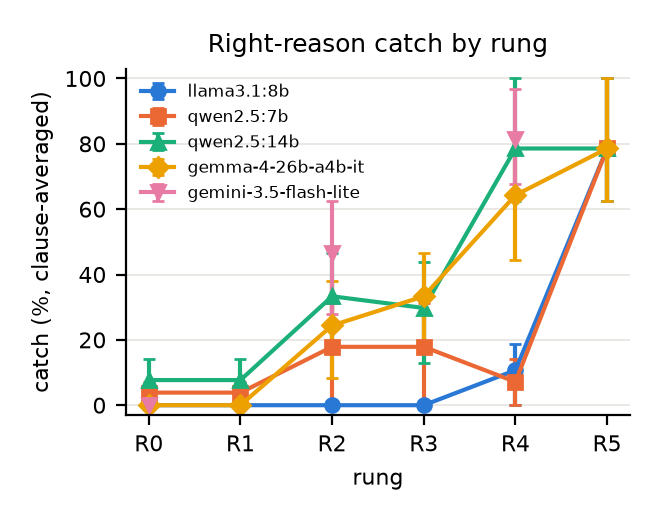
\includegraphics[width=0.7\linewidth]{generated/fig_ladder.png}
\caption{Right-reason catch by rung, one line per model, clause-averaged, with \CILevel\% bootstrap intervals
over clauses. \rung{R5} is the registry lookup and is the same for every model.}
\label{fig:ladder}
\end{figure}

\begin{table*}[t]
\centering
\footnotesize
\setlength{\tabcolsep}{2pt}
\begin{tabular}{l ccc ccc ccc ccc}
\toprule
& \multicolumn{3}{c}{\texttt{llama3.1:8b}} & \multicolumn{3}{c}{\texttt{qwen2.5:7b}}
& \multicolumn{3}{c}{\texttt{qwen2.5:14b}} & \multicolumn{3}{c}{\texttt{gemma-4-26b}} \\
\cmidrule(lr){2-4}\cmidrule(lr){5-7}\cmidrule(lr){8-10}\cmidrule(lr){11-13}
Rung & Catch & FA-m & FA-C & Catch & FA-m & FA-C & Catch & FA-m & FA-C & Catch & FA-m & FA-C \\
\midrule
\rung{R0} & \CatchLlamaRZero & \FAMLlamaRZero & \FACLlamaRZero & \CatchQwenSevenRZero & \FAMQwenSevenRZero & \FACQwenSevenRZero & \CatchQwenFourteenRZero & \FAMQwenFourteenRZero & \FACQwenFourteenRZero & \CatchGemmaRZero & \FAMGemmaRZero & \FACGemmaRZero \\
\rung{R1} & \CatchLlamaROne & \FAMLlamaROne & \FACLlamaROne & \CatchQwenSevenROne & \FAMQwenSevenROne & \FACQwenSevenROne & \CatchQwenFourteenROne & \FAMQwenFourteenROne & \FACQwenFourteenROne & \CatchGemmaROne & \FAMGemmaROne & \FACGemmaROne \\
\rung{R2} & \CatchLlamaRTwo & \FAMLlamaRTwo & \FACLlamaRTwo & \CatchQwenSevenRTwo & \FAMQwenSevenRTwo & \FACQwenSevenRTwo & \CatchQwenFourteenRTwo & \FAMQwenFourteenRTwo & \FACQwenFourteenRTwo & \CatchGemmaRTwo & \FAMGemmaRTwo & \FACGemmaRTwo \\
\rung{R3} & \CatchLlamaRThree & \FAMLlamaRThree & \FACLlamaRThree & \CatchQwenSevenRThree & \FAMQwenSevenRThree & \FACQwenSevenRThree & \CatchQwenFourteenRThree & \FAMQwenFourteenRThree & \FACQwenFourteenRThree & \CatchGemmaRThree & \FAMGemmaRThree & \FACGemmaRThree \\
\rung{R4} & \CatchLlamaRFour & \FAMLlamaRFour & \FACLlamaRFour & \CatchQwenSevenRFour & \FAMQwenSevenRFour & \FACQwenSevenRFour & \CatchQwenFourteenRFour & \FAMQwenFourteenRFour & \FACQwenFourteenRFour & \CatchGemmaRFour & \FAMGemmaRFour & \FACGemmaRFour \\
\Rfourp & \CatchLlamaRFourP & \FAMLlamaRFourP & \FACLlamaRFourP & \CatchQwenSevenRFourP & \FAMQwenSevenRFourP & \FACQwenSevenRFourP & \CatchQwenFourteenRFourP & \FAMQwenFourteenRFourP & \FACQwenFourteenRFourP & \CatchGemmaRFourP & \FAMGemmaRFourP & \FACGemmaRFourP \\
\rung{R5} & \CatchLlamaRFive & \FAMLlamaRFive & \FACLlamaRFive & \CatchQwenSevenRFive & \FAMQwenSevenRFive & \FACQwenSevenRFive & \CatchQwenFourteenRFive & \FAMQwenFourteenRFive & \FACQwenFourteenRFive & \CatchGemmaRFive & \FAMGemmaRFive & \FACGemmaRFive \\
\bottomrule
\end{tabular}
\caption{Right-reason catch and false alarms by rung (clause-averaged; C false alarms averaged by rule group).
FA-m: matched correct answers of the same blocks (S-swap pairs for \rung{R0}, \rung{R1} and \Rfourp, S-both
otherwise; \rung{R5} pools both). FA-C: clean correct answers. Table~\ref{tab:main} gives S-both counts only, so its
false alarms can differ from FA-m here.}
\label{tab:ladder}
\end{table*}

The ladder is the reference that places Q1 and Q2. For both capable models the status line lifted right-reason
catches over seeing both versions: \rung{R4}$-$\rung{R2} was \DiffRFourMinusRTwoQwenFourteen{} points for
\texttt{qwen2.5:14b} (CI \CIRFourMinusRTwoQwenFourteen) and \DiffRFourMinusRTwoGemma{} for Gemma (CI
\CIRFourMinusRTwoGemma), while \rung{R2}$-$\rung{R0} was \DiffRTwoMinusRZeroQwenFourteen{} and
\DiffRTwoMinusRZeroGemma{} (on the \ClausesRTwoMinusRZeroGemma{} clauses where both rungs ran, so they differ from the
clause averages of Table~\ref{tab:ladder}), not significant by the planned sign-flip test (Gemma's bootstrap interval,
\CIRTwoMinusRZeroGemma, excludes zero; \rung{R0} runs on S-swap items, where a right-reason catch is near zero by
design). In the words fixed in advance, seeing both versions is not enough, and
\rung{R4} lifts these capable models. The amending instrument's quote (\rung{R3}) added little over \rung{R2}
(\DiffRThreeMinusRTwoQwenFourteen{} and \DiffRThreeMinusRTwoGemma{} points). Without a record the reviewers did
not discriminate at all: \rung{R2} discrimination was \DiscRTwoQwenFourteen{} points for \texttt{qwen2.5:14b} and
\DiscRTwoGemma{} for Gemma, because they flagged matched correct answers as often as, or more often than, they caught faults for
the right reason.

The weak model gained little: \texttt{llama3.1:8b} caught \CatchLlamaRTwo{} at \rung{R2} and \CatchLlamaRFour{} at
\rung{R4} (\DiffRFourMinusRTwoLlama{} points, interval \CIRFourMinusRTwoLlama). That is just outside the
\InterpPoints-point margin of the reading fixed in advance for this case (reading 12), so that reading does not apply;
we report the small gain as a limit of the claim. \texttt{gemini-3.5-flash-lite}, run at \rung{R0}, \rung{R2} and \rung{R4} only, caught
\CatchFlashRTwo{} at \rung{R2} and \CatchFlashRFour{} at \rung{R4}, with false alarms on matched correct answers
of \FAMFlashRFour{} at \rung{R4}; seeing both versions did not close the gap for it either. Given the ``can't confirm'' option (E2), neither capable model used it on a fault at \rung{R2}
(\CantConfirmKNQwenFourteenRTwoCC{} and \CantConfirmKNGemmaRTwoCC): the option was available and unused. Of the
\rung{R2} findings that flagged the replaced clause, \MisnamedKNQwenFourteenRTwo{} (\texttt{qwen2.5:14b}) and
\MisnamedKNGemmaRTwo{} (Gemma) never gave ``not in force'' as the reason (E4).

\subsubsection{The added models}
\label{sec:res-explore}
\IfFileExists{generated/tab_exploratory.tex}{\begin{table}[t]\centering\small
\caption{The two models added after the plan: a size comparison within one family, and Claude Opus 4.5. Rows marked ``no'' were added after the analysis plan was fixed and are exploratory; the planned sizes are shown beside them. The 32B model ran damage seeds 0--2 (the planned capable models ran 0--4). S-both right-reason catches, false alarms on matched correct answers (any finding) and any-finding catches, pooled k/n; discrimination clause-averaged (points), and the Q1 difference with a 95\% bootstrap interval over clauses. No test.}
\label{tab:exploratory}
\footnotesize\setlength{\tabcolsep}{3pt}
\begin{tabular}{lllrrrl}
\toprule
Model & Planned & Arm & Catch & FA & Any & Disc. / diff. \\
\midrule
Qwen 7B & yes & R2 & 5/42 & 7/42 & 14/42 & $-$1 \\
Qwen 7B & yes & R4 & 2/42 & 2/42 & 3/42 & +0 \\
Qwen 7B & yes & R4-drop50 & 2/42 & 2/42 & 3/42 & +0 \\
Qwen 7B & yes & R4$-$R5, intact & \multicolumn{3}{c}{} & $-$67 [$-$88, $-$43] \\
Qwen 7B & yes & R4$-$R5, drop50 & \multicolumn{3}{c}{} & $-$42 [$-$60, $-$24] \\
\addlinespace
Qwen 14B & yes & R2 & 13/42 & 18/42 & 26/42 & $-$7 \\
Qwen 14B & yes & R4 & 32/42 & 10/42 & 32/42 & +55 \\
Qwen 14B & yes & R4n & 31/42 & 13/42 & 32/42 & +47 \\
Qwen 14B & yes & R4-drop50 & 88/210 & 54/210 & 126/210 & +21 \\
Qwen 14B & yes & R4$-$R5, intact & \multicolumn{3}{c}{} & $-$11 [$-$33, +9] \\
Qwen 14B & yes & R4$-$R5, drop50 & \multicolumn{3}{c}{} & $-$21 [$-$38, $-$6] \\
\addlinespace
Qwen 32B & no & R2 & 4/42 & 25/42 & 35/42 & $-$48 \\
Qwen 32B & no & R4 & 29/42 & 23/42 & 38/42 & +18 \\
Qwen 32B & no & R4n & 26/42 & 24/42 & 38/42 & +11 \\
Qwen 32B & no & R4-drop50 & 46/126 & 69/126 & 104/126 & $-$15 \\
Qwen 32B & no & R4$-$R5, intact & \multicolumn{3}{c}{} & $-$48 [$-$68, $-$24] \\
Qwen 32B & no & R4$-$R5, drop50 & \multicolumn{3}{c}{} & $-$57 [$-$76, $-$37] \\
\addlinespace
Claude Opus 4.5 & no & R2 & 34/42 & 40/42 & 42/42 & $-$11 \\
Claude Opus 4.5 & no & R4 & 35/42 & 37/42 & 42/42 & $-$3 \\
Claude Opus 4.5 & no & R4n & 35/42 & 42/42 & 42/42 & $-$14 \\
Claude Opus 4.5 & no & R4-drop50 & 29/42 & 37/42 & 42/42 & $-$21 \\
Claude Opus 4.5 & no & R4$-$R5, intact & \multicolumn{3}{c}{} & $-$70 [$-$89, $-$48] \\
Claude Opus 4.5 & no & R4$-$R5, drop50 & \multicolumn{3}{c}{} & $-$63 [$-$85, $-$43] \\
\bottomrule
\end{tabular}
\end{table}
}{}
The two models added after the analysis plan was fixed are outside every planned test; Table~\ref{tab:exploratory}
and the descriptive-results table of the paper's case-study appendix report them on the main arms. Claude Opus~4.5
behaves differently from the open models: it is the only reviewer whose catches survive the absence of a record, and
the one with the clearest net gain against the damaged lookup (gaining many and losing none). Its catches on dropped links still
fell under the damaged status line, as in the main study, and its false alarms on this key's correct answers are
the highest; against a flawed key they cannot be interpreted. A model from the same developer also helped build this
benchmark (see the paper's statement on the use of AI assistants); its items were not tuned on any model's replies,
but readers should weigh that relation. It ran one damage seed, through a
proxy that sets temperature and seed itself, so its numbers carry more uncertainty than the planned models'. In the one family we ran at three sizes, the largest model did not review better than the 14B one: \texttt{qwen2.5:32b}, run with
the pre-specified prompts on the same items, flagged matched correct answers more often than
\texttt{qwen2.5:14b} at every arm, and about twice as often once given the record, so its discrimination was lower, and its gap to the lookup wider, with the record
intact and with half the links dropped. Without a record it named the replaced clause on most faults but rarely for
the reason that it is no longer in force. On the dropped-link faults its catches fell to none under the damaged
status line, and the no-record wording did not restore them. One model, one family and the same \NClauses{} clauses
cannot separate size from other differences between checkpoints; we report it because a reader will ask whether a
larger model removes the pattern, and here it did not.

\subsubsection{Sensitivity to the annotation audit}
\label{sec:res-sens}
Removing the cases whose checked correct answer annotators judged flawed (S1; only a sample was checked) left the sign
of every primary contrast unchanged (Table~\ref{tab:provenance}). Gemma's two significant Q1 differences became
\SOneDiffNetIntactGemma{} and \SOneDiffNetSpuriousTenGemma{} points with Holm $p=$ \SOnePHolmNetIntactGemma{} and
\SOnePHolmNetSpuriousTenGemma, no longer below \Alpha{} on the smaller set. Under the reading fixed in advance, the
direction of the Q1 result does not depend on the correct answers known to be flawed; its significance for Gemma does
depend on keeping them. Under the original strict rule (S2) only \NStrictKept{} cases remain, on fewer than \MinClauses{} clauses; that
is descriptive only, and there \texttt{qwen2.5:14b}'s Q1 difference turns positive (\STwoDiffNetIntactQwenFourteen{}
points intact), Gemma's stays negative (\STwoDiffNetIntactGemma).

